\documentclass[12pt]{article}

\pagestyle{empty}
\setcounter{secnumdepth}{2}

\topmargin=-1.5cm
\oddsidemargin=0cm
\textheight=23.0cm
\textwidth=16cm
\parindent=0cm
\parskip=0.15cm
\topskip=0truecm
\raggedbottom
\abovedisplayskip=3mm
\belowdisplayskip=3mm
\abovedisplayshortskip=0mm
\belowdisplayshortskip=2mm
\normalbaselineskip=12pt
\normalbaselines

\usepackage{tabularx}
\usepackage{multirow}
\usepackage{indentfirst}

% Making \cellwidth the width of the tabularx cell we are currently in
\makeatletter
\newcommand{\cellwidth}{\TX@col@width}
\makeatother

\usepackage{graphicx}
\graphicspath{{.}}
\DeclareGraphicsExtensions{.png}

\usepackage{float}
\restylefloat{table}
\usepackage{color}
\usepackage{hyperref}
\hypersetup{
  colorlinks=true, 
  linkcolor=blue, 
  filecolor=magenta,
  urlcolor=cyan,
}

\urlstyle{same}

\begin{document}

\vspace*{0.5in}
\centerline{\bf\Large User Requirements Document}

\vspace*{0.5in}
\centerline{\bf\Large Team T}

\vspace*{0.5in}
\centerline{\bf\Large February 3\textsuperscript{rd} 2016}

\vspace*{1.5in}
\begin{table}[htbp]
\caption{Team}
\begin{center}
\begin{tabular}{|r | c|}
\hline
Name & ID Number \\
\hline\hline
Lenmor Larroza Dimanalata & 27699727 \\
\hline
Andrea Julia Biondi & 26456251 \\
\hline
Jonathan Roux & 26978185 \\
\hline
Andres Kebe & 26638422 \\
\hline
Matin Nafekh & 27423993 \\
\hline
Sebastien Seguier & 27010699 \\
\hline
Erick Hernandez & 27083181 \\
\hline
Haochen Wang & 26414249 \\
\hline

\end{tabular}
\end{center}
\end{table}

\clearpage
\begin{table}
\centerline{\bf\Large Revision History}
\begin{center}
\begin{tabular}{|l | l| l|l|}
\hline
\bf Date & \bf Version & \bf Description & \bf Author \\
\hline
19/01/2016 & 1.0 & Document Start & Jonathan Roux \\
\hline
23/01/2016 & 1.1 & Use Cases added & Jonathan Roux \\
\hline
24/01/2016 & 1.2 & Use Case Diagram & Jonathan Roux \\
\hline
27/01/2016 & 1.3 & Domain Concepts & Jonathan Roux \\
\hline
27/01/2016 & 1.4 & User Groups, Functional Req. & Andrea Julia Biondi \\
\hline
28/01/2016 & 1.5 & Functional Req., System Overview & Andrea Julia Biondi \\
\hline
01/02/2016 & 1.6 & Brief modifications (Use Cases, Requirements) & Andrea Julia Biondi \\
\hline
02/02/2016 & 1.7 & Modification in functional req., References & Andrea Julia Biondi \\
\hline
02/02/2016 & 1.8 & 2 new use cases and update use case diagram & Jonathan Roux \\
\hline

\end{tabular}
\end{center}
\end{table}

\clearpage

\tableofcontents

\clearpage

\section{Purpose of the document}
The purpose of this document is to describe all the necessary requirements for the development of a 1D-2D GCHQ Puzzle Application.
It is intended for review by the Britain's security and intelligence organization GCHQ
\begin{table}[htbp]
\caption{Intended audience of this document}
\begin{center}
\begin{tabular}{|l | l|}
\hline
Group & Intended purposes \\
\hline\hline
Puzzle makers and solvers & To help coders review the application \\
\hline
Coders & To know the different components for the application \\
\hline
Testers & To test whether the application meets the requirements \\
\hline
Writers of related documents & To use as a reference for future deliverable\\
\hline
\end{tabular}
\end{center}
\end{table}

\section{Business Goals}
\setlength{\parindent}{5ex}

The 1D-2D GCHQ Puzzle is simple, but requires a fair amount of computation to obtain and solve. The main goals of this project can be separated in two categories: a tool to make puzzles
with different settings, and a GUI with many options for puzzle solvers.

A puzzle is meant to be challenging and since different users prefer different challenges, a puzzle maker will be able to create puzzles of different sizes and level 
of difficulty. Also, the assignment of priorities can be applied to rows and columns to help the puzzle solvers. Moreover, the puzzle maker will be able to inform the puzzle solvers
when some row or column has all its conditions met.

From the perspective of a puzzle solver, the application will be an intuitive GUI that will allow easy visualisation, manipulation and modification of the puzzle. One of the principal functions
of this program is that it will determine if the current grid is a solution or not. Also, given some state of the grid the puzzle solver will be able to consider different solutions simultaneously.


\section{Domain Concepts}

\begin{figure}[H]
\begin{center}
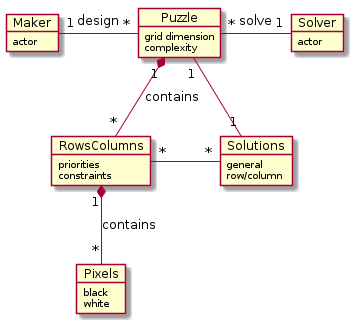
\includegraphics[scale=0.6]{classdiagram}
\caption{UML Class Diagram}
\label{fig:class-diagram}
\end{center}
\end{figure}

\begin{table}[H]
\caption{Main Domain concept of the 1D-2D Puzzle}
\begin{center}
\begin{tabularx}{\textwidth}{|p{1.75cm} | X|}
\hline
\bf Concept & \bf Description \\
\hline
Puzzle & This is the central concept of this project. All other domain concepts are related in some way to the puzzle concept. It is composed of rows and columns which are determined by the grid dimension attribute.
The complexity attribute describe how many starting pixels will be available to the puzzle solver. \\
\hline
Rows and Columns & The puzzle can be decomposed into rows and columns, each one with its own constraints and priorities. The constraints determine the number and length of black pixel runs. The priorities is extra
information about which row or column to solve first to help the puzzle solver.\\
\hline
Pixels & This is the most basic component of the puzzle and is either black or white. The goal is to determine which pixels are black so all the constraints are satisfied. \\
\hline
Solution & This is the configuration of the puzzle when all the constraints for each rows and columns are satisfied. There is also intermediary solution, when a configuration is satisfied only for a specific 
row or column. More than one solution is possible for a given puzzle. \\
\hline
Puzzle Maker & This is the actor who will determine the configuration of the puzzle: dimension, complexity, constraints and priorities on rows and columns. \\
\hline
Puzzle Solver & This is the actor who will try to find the initial configuration of the puzzle given some initial black pixels and respecting the constraints. Some extra information about priorities 
on some rows or columns may also be available. \\
\hline
\end{tabularx}
\end{center}
\end{table}

\section{System overview}
\setlength{\parindent}{5ex}
 
 
This system allows users to create or solve puzzles. These users will be using the systems' GUI in order to display the features they can use.

The puzzle maker is allowed to create a puzzle which can vary of size and difficulty. While the puzzle is being created, the system can allow different priorities to be set for the puzzle. In addition to these features, the system can identify different possibilities for a puzzle solution. 

The puzzle solver has features that include assigning black or white pixels in the grid of the puzzle, verifying if the grid is a correct solution, and manipulating certain regions to maximize their ability to find a solution.

\section{User groups}
\begin{table}[htbp]
\caption{Users of the system}
\begin{center}
\begin{tabular}{|l | l| c|}
\hline
\textbf{Users} & \textbf{Description} & \textbf{Number of Users}\\
\hline\hline
Puzzle Maker & Those who create the puzzles & 1 \\
\hline
Puzzle Solver & Those who solve the puzzles & 1 \\
\hline
\end{tabular}
\end{center}
\end{table}

\clearpage

\section{Functional requirements}
\begin{table}[htbp]
\caption{Functional}
\begin{center}
%\begin{tabular}{|l | l| l| l| l|}
\begin{tabularx}{\textwidth}{|p{0.4cm} | p{1.5cm}| X| p{3.35cm}| c| c|}
\hline
\textbf{ID} & \textbf{Feature} & \textbf{Requirement} & \textbf{Rationale} & \textbf{Priority} & \textbf{Use Case}\\
\hline\hline
01 & Opening & Any user shall be able to open the application & There is no login required & Must & 1\\
\hline
02 & Opening & User shall be able to choose between creating and solving puzzle & User can be both maker and solver, but only one at a time & Must & 1 \\
\hline
03 & Creating & Puzzle maker shall be able to set number of rows and columns & User adjusts the size based on level of difficulty  & Must & 2 \\
\hline
04 & Creating & Puzzle maker shall be able to set black pixels in puzzle & The pixels are placed in order to complete the puzzle & Must & 2 \\
\hline
05 & Creating & Puzzle maker shall be able to modify the size of black regions & Constraints will be added according to the black regions & Must & 3 \\
\hline
06 & Confirmation & The system must be able to confirm if a puzzle has been solved quickly & An optional feature that is used by the puzzle maker & Must & 3 \\
\hline
07 & Creating & User shall be able to add priorities to rows/columns & The priorities guide the puzzle solver & Must & 4 \\
\hline
08 & Solving & Puzzle solver shall be able to identify different possibilities of solutions & Allows the solver to find new solutions & Must & 5 \\
\hline
09 & Solving & Puzzle solver shall be able to manipulate specific regions in solution & User can drag regions in different directions to change solution & Must & 6 \\
\hline
\end{tabularx}
\end{center}
\end{table}

\clearpage

\section{Non-functional requirements (quality requirements, properties)}

\begin{table}[htbp]
\caption{Non-Functional Requirements}
\begin{center}
\begin{tabularx}{\textwidth}{|p{0.75cm} | X| X| c| c|}
\hline
\textbf{ID} & \textbf{Requirement} & \textbf{Rationale} & \textbf{Priority} & \textbf{Use Case}\\
\hline\hline
01  & Portability & As many users as possible must be able to play the game & Must & -\\
\hline
02  & Response Time & Each time the puzzle solver click a pixels the system has to check if the constraints are satisfied & Must & 3 \\
\hline
03  & Accessibility & Puzzles of different sizes and complexity must be available to the puzzle solver  & Must & 2 \\
\hline
04  & Performance & Regardless of the size of the puzzle, the system must check the solution under a second & Must & 3 \\
\hline
05  & Reliability & Neither the solver or the maker want the application to crash  & Must & All \\
\hline
06  & Extensibility & New ideas from users must be able to be easily implemented to the system & Must & - \\
\hline
\end{tabularx}
\end{center}
\end{table}

\clearpage

\section{Use Cases}

\subsection{Overview}

\begin{figure}[H]
\begin{center}
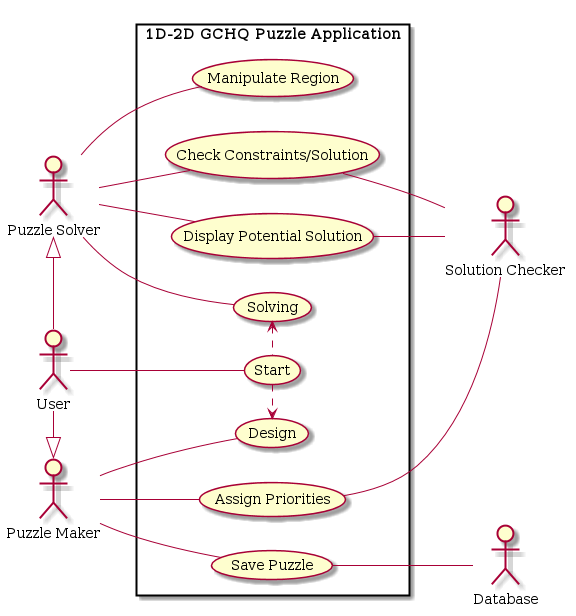
\includegraphics[scale=0.5]{usecasediagram}
\caption{Use Case Diagram}
\label{fig:use-case-diagram}
\end{center}
\end{figure}

\subsection{Use Case 1} \label{uc:1}

\begin{table}[H]
\begin{center}
\begin{tabularx}{\textwidth}{|p{3.3cm} | X|}
\hline
\bf Name & Start \\
\hline
\bf Summary & The user open the application.\\
\hline
\bf Actors & Any user. \\
\hline
\bf Preconditions & - \\
\hline
\bf Basic Sequence & {\begin{tabularx}{\cellwidth} {@{}X@{}} 1. A user starts the application. \\ 
2. The user decides whether he wants to make or solve puzzles by clicking on the right button. \\ \end{tabularx}} \\
\hline
\bf Exceptions & - \\
\hline
\bf Post Conditions & A user will be either a puzzle maker or puzzle solver. \\
\hline
\bf Priority & Must \\
\hline
\bf Status & Implemented \\
\hline
\bf Traces to requirements & - \\
\hline
\bf Traces to test cases & reference to test cases \\
\hline
\end{tabularx}
\end{center}
\end{table}

\clearpage

\subsection{Use Case 2} \label{uc:2}


\begin{table}[H]
\begin{center}
\begin{tabularx}{\textwidth}{|p{3.3cm} | X|}
\hline
\bf Name & Design \\
\hline
\bf Summary & The puzzle maker creates a puzzle.\\
\hline
\bf Actors & Puzzle maker \\
\hline
\bf Preconditions & The user is a puzzle maker starting the creation of a new puzzle. \\
\hline
\bf Basic Sequence & {\begin{tabularx}{\cellwidth} {@{}X@{}} 1. The puzzle maker is requested to enter the number of rows and columns for its next puzzle. \\ 
2. The system generates an empty grid using the specified number of rows and columns. \\
3. The puzzle maker chooses which pixels are black or white by clicking them. \\
4. When done, the puzzle maker is requested to determine the black pixels that will be available to the puzzle solver as hints. \\
\end{tabularx}} \\
\hline
\bf Exceptions & {\begin{tabularx}{\cellwidth} {@{}X@{}} 1a. If the number of rows or columns is too large, the message "Number of Rows/Columns too large" will be displayed \\ 
1b. If the number of rows of columns is too small, the message "Number of Rows/Coumns must be equal or greater than 4" will be displayed \\
\end{tabularx}} \\
\hline
\bf Post Conditions & A new puzzle was created. \\
\hline
\bf Priority & Must \\
\hline
\bf Status & Implemented \\
\hline
\bf Traces to requirements & User Story \#1 \\
\hline
\bf Traces to test cases & reference to test cases \\
\hline
\end{tabularx}
\end{center}
\end{table}

\clearpage

\subsection{Use Case 3} \label{uc:3}

\begin{table}[H]
\begin{center}
\begin{tabularx}{\textwidth}{|p{3.3cm} | X|}
\hline
\bf Name & Solving \\
\hline
\bf Summary & The puzzle solver solves a puzzle.\\
\hline
\bf Actors & The puzzle solver, Solution Checker \\
\hline
\bf Preconditions & The user is a puzzle solver. \\
\hline
\bf Basic Sequence & {\begin{tabularx}{\cellwidth} {@{}X@{}} 1. The puzzle solver chooses a puzzle by size and complexity. \\
2. The puzzle solver can modify the color of the pixels to either black or white by clicking them. \\ 
3. The puzzle solver can click the button "Check", when he thinks he has the right answer. \\ 
4. The solution checker has to check if the configuration of the grid satisfies all the constraints of the puzzle.\\ 
5. The system congratulates the puzzle solver. \end{tabularx}} \\
\hline
\bf Exceptions & {\begin{tabularx}{\cellwidth} {@{}X@{}} 3a. If the configuration of the grid is not right, the puzzle solver can keep on trying and re-submit later. \\ 
\end{tabularx}} \\
\hline
\bf Post Conditions & The puzzle solver solved a puzzle. \\
\hline
\bf Priority & Must \\
\hline
\bf Status & Implemented \\
\hline
\bf Traces to requirements & User Story \ 2,3 \\
\hline
\bf Traces to test cases & reference to test cases \\
\hline
\end{tabularx}
\end{center}
\end{table}

\clearpage


\subsection{Use Case 4} \label{uc:4}

\begin{table}[H]
\begin{center}
\begin{tabularx}{\textwidth}{|p{3.3cm} | X|}
\hline
\bf Name & Assign Priorities \\
\hline
\bf Summary & The puzzle maker can decide to assign priorities to rows/columns to guide the puzzle solver.\\
\hline
\bf Actors & Puzzle Solver, Solution Checker\\
\hline
\bf Preconditions & The puzzle maker designs a puzzle. \\
\hline
\bf Basic Sequence & {\begin{tabularx}{\cellwidth} {@{}X@{}} 1. While designing the puzzle, the puzzle maker can decide to give priorities to some rows/columns to be solved by the puzzle solver. \\ 
2. The solution checker will analyse the puzzle and determine which rows/columns should be solved first by the puzzle solver. \end{tabularx}} \\
\hline
\bf Exceptions & {\begin{tabularx}{\cellwidth} {@{}X@{}} 2a. If the puzzle maker updates the puzzle, he should reassign priorities to rows/columns according to the new configuation. \\ \end{tabularx}} \\
\hline
\bf Post Conditions & The puzzle maker can keep on designing the puzzle. \\
\hline
\bf Priority & Must \\
\hline
\bf Status & In progress \\
\hline
\bf Traces to requirements & User Story \#4 \\
\hline
\bf Traces to test cases & reference to test cases \\
\hline
\end{tabularx}
\end{center}
\end{table}

\clearpage

\subsection{Use Case 5} \label{uc:5}

\begin{table}[H]
\begin{center}
\begin{tabularx}{\textwidth}{|p{3.3cm} | X|}
\hline
\bf Name & Display Potential Solutions \\
\hline
\bf Summary & The puzzle solver can see the different solutions for a given row or column.\\
\hline
\bf Actors & Puzzle solver \\
\hline
\bf Preconditions & The puzzle solver is working out the puzzle. \\
\hline
\bf Basic Sequence & {\begin{tabularx}{\cellwidth} {@{}X@{}} 1. The puzzle solver can select an entire row or column. \\ 
2. The system identifies and displays the different possibilities for black pixels for this particular row or column according to the current configuation of the puzzle. \\ \end{tabularx}} \\
\hline
\bf Exceptions & {\begin{tabularx}{\cellwidth} {@{}X@{}} -  \\ \end{tabularx}} \\
\hline
\bf Post Conditions & The puzzle solver may try one of displayed solutions for the given row/column. \\
\hline
\bf Priority & Must \\
\hline
\bf Status & In progress \\
\hline
\bf Traces to requirements & User Story \#5 \\
\hline
\bf Traces to test cases & reference to test cases \\
\hline
\end{tabularx}
\end{center}
\end{table}

\clearpage

\subsection{Use Case 6} \label{uc:10}

\begin{table}[H]
\begin{center}
\begin{tabularx}{\textwidth}{|p{3.3cm} | X|}
\hline
\bf Name & Manipulate Region \\
\hline
\bf Summary & The puzzle solver can move entire regions of black pixels horizontally for a row or vertically for a column. \\
\hline
\bf Actors & Puzzle solver \\
\hline
\bf Preconditions & The puzzle solver is working out the puzzle. \\
\hline
\bf Basic Sequence & {\begin{tabularx}{\cellwidth} {@{}X@{}} 1. The puzzle solver can click on a black pixel. \\ 
2. The system can recognize if the clicked pixels has other adjacent black pixels forming a block. \\
3. The puzzle solver can drag this block either horizontally or vertically and permanently change the position of the whole block. \end{tabularx}} \\
\hline
\bf Exceptions & {\begin{tabularx}{\cellwidth} {@{}X@{}} -  \\ \end{tabularx}} \\
\hline
\bf Post Conditions & The puzzle solver can keep on working out the puzzle. \\
\hline
\bf Priority & Must \\
\hline
\bf Status & In progress \\
\hline
\bf Traces to requirements & User Story \#7 \\
\hline
\bf Traces to test cases & reference to test cases \\
\hline
\end{tabularx}
\end{center}
\end{table}

\clearpage

\subsection{Use Case 7} \label{uc:3}

\begin{table}[H]
\begin{center}
\begin{tabularx}{\textwidth}{|p{3.3cm} | X|}
\hline
\bf Name & Check Constraints \\
\hline
\bf Summary & The Solution Checker checks in real-time if some row or column constraints are satisfied. \\
\hline
\bf Actors & The puzzle solver, Solution Checker \\
\hline
\bf Preconditions & The user is a puzzle solver solving a puzzle. \\
\hline
\bf Basic Sequence & {\begin{tabularx}{\cellwidth} {@{}X@{}} 1. The puzzle solver clicks on a pixel, changing the configuration of the grid. \\
2. The Solution Checker highlights the constraints that are satisfied. \\
3. If some row or column have all their constraints satisfied, the entire row/column will be highlighted. \end{tabularx}} \\
\hline
\bf Exceptions & {\begin{tabularx}{\cellwidth} {@{}X@{}} 2a. If a modification in the configuration of the grid loses a previously satisfied constraint, then the Solution Checker will remove the highlight on the constraint. \\ 
3a. If a modification in the configuration of the grid loses a previously satisfied row/column, then the Solution Checker will remove the highlight on the entire row/column. \end{tabularx}} \\
\hline
\bf Post Conditions & The puzzle solver can visualize the current status of its puzzle.  \\
\hline
\bf Priority & Optional \\
\hline
\bf Status & In progress \\
\hline
\bf Traces to requirements & User Story \#6 \\
\hline
\bf Traces to test cases & reference to test cases \\
\hline
\end{tabularx}
\end{center}
\end{table}

\clearpage

\subsection{Use Case 8} \label{uc:2}


\begin{table}[H]
\begin{center}
\begin{tabularx}{\textwidth}{|p{3.3cm} | X|}
\hline
\bf Name & Save Puzzle \\
\hline
\bf Summary & The puzzle maker saves a puzzle to a database.\\
\hline
\bf Actors & Puzzle maker, Database \\
\hline
\bf Preconditions & The puzzle maker finished the creation of a new puzzle. \\
\hline
\bf Basic Sequence & {\begin{tabularx}{\cellwidth} {@{}X@{}} 1. The puzzle maker can save the configuration of the new puzzle. \\ 
2. The system will assign and id to the puzzle and save it in a database. \end{tabularx}} \\
\hline
\bf Exceptions & - \\
\hline
\bf Post Conditions & A new puzzle was created and saved to a database. \\
\hline
\bf Priority & Must \\
\hline
\bf Status & In progress \\
\hline
\bf Traces to requirements & User Story \#1 \\
\hline
\bf Traces to test cases & reference to test cases \\
\hline
\end{tabularx}
\end{center}
\end{table}

\clearpage

\section{References}
\textbf{User Stories:}

\begin{itemize}
\item \textbf{US 1:} As a puzzle maker, I want to create puzzles of different sizes and complexity with the application.
\item \textbf{US 2:} As a puzzle solver, I want to assign black-white values to pixels in the grid of the puzzle.
\item \textbf{US 3:} As a puzzle solver, I want to check whether my current grid is a solution or not.
\item \textbf{US 4:} As a puzzle maker, I want to assign priorities to rows and columns of the puzzle grid to guide the puzzle solver
\item \textbf{US 5:} As a puzzle solver, I want to simultaneously consider several potential solutions for a row (or a column).
\item \textbf{US 6:} As a puzzle maker, I want to inform the puzzle solver when there is a row or column that fully determined by the current state of the puzzle grid.
\item \textbf{US 7:} As a puzzle solver, I want to be able to manipulate entire regions in a potential solutions for a row (or a column) by dragging them horizontally (or vertically).
\end{itemize}

\end{document}
